\section{Hardware}

Overview text required.





\subsection{PCB Stack Layout}

\begin{center}
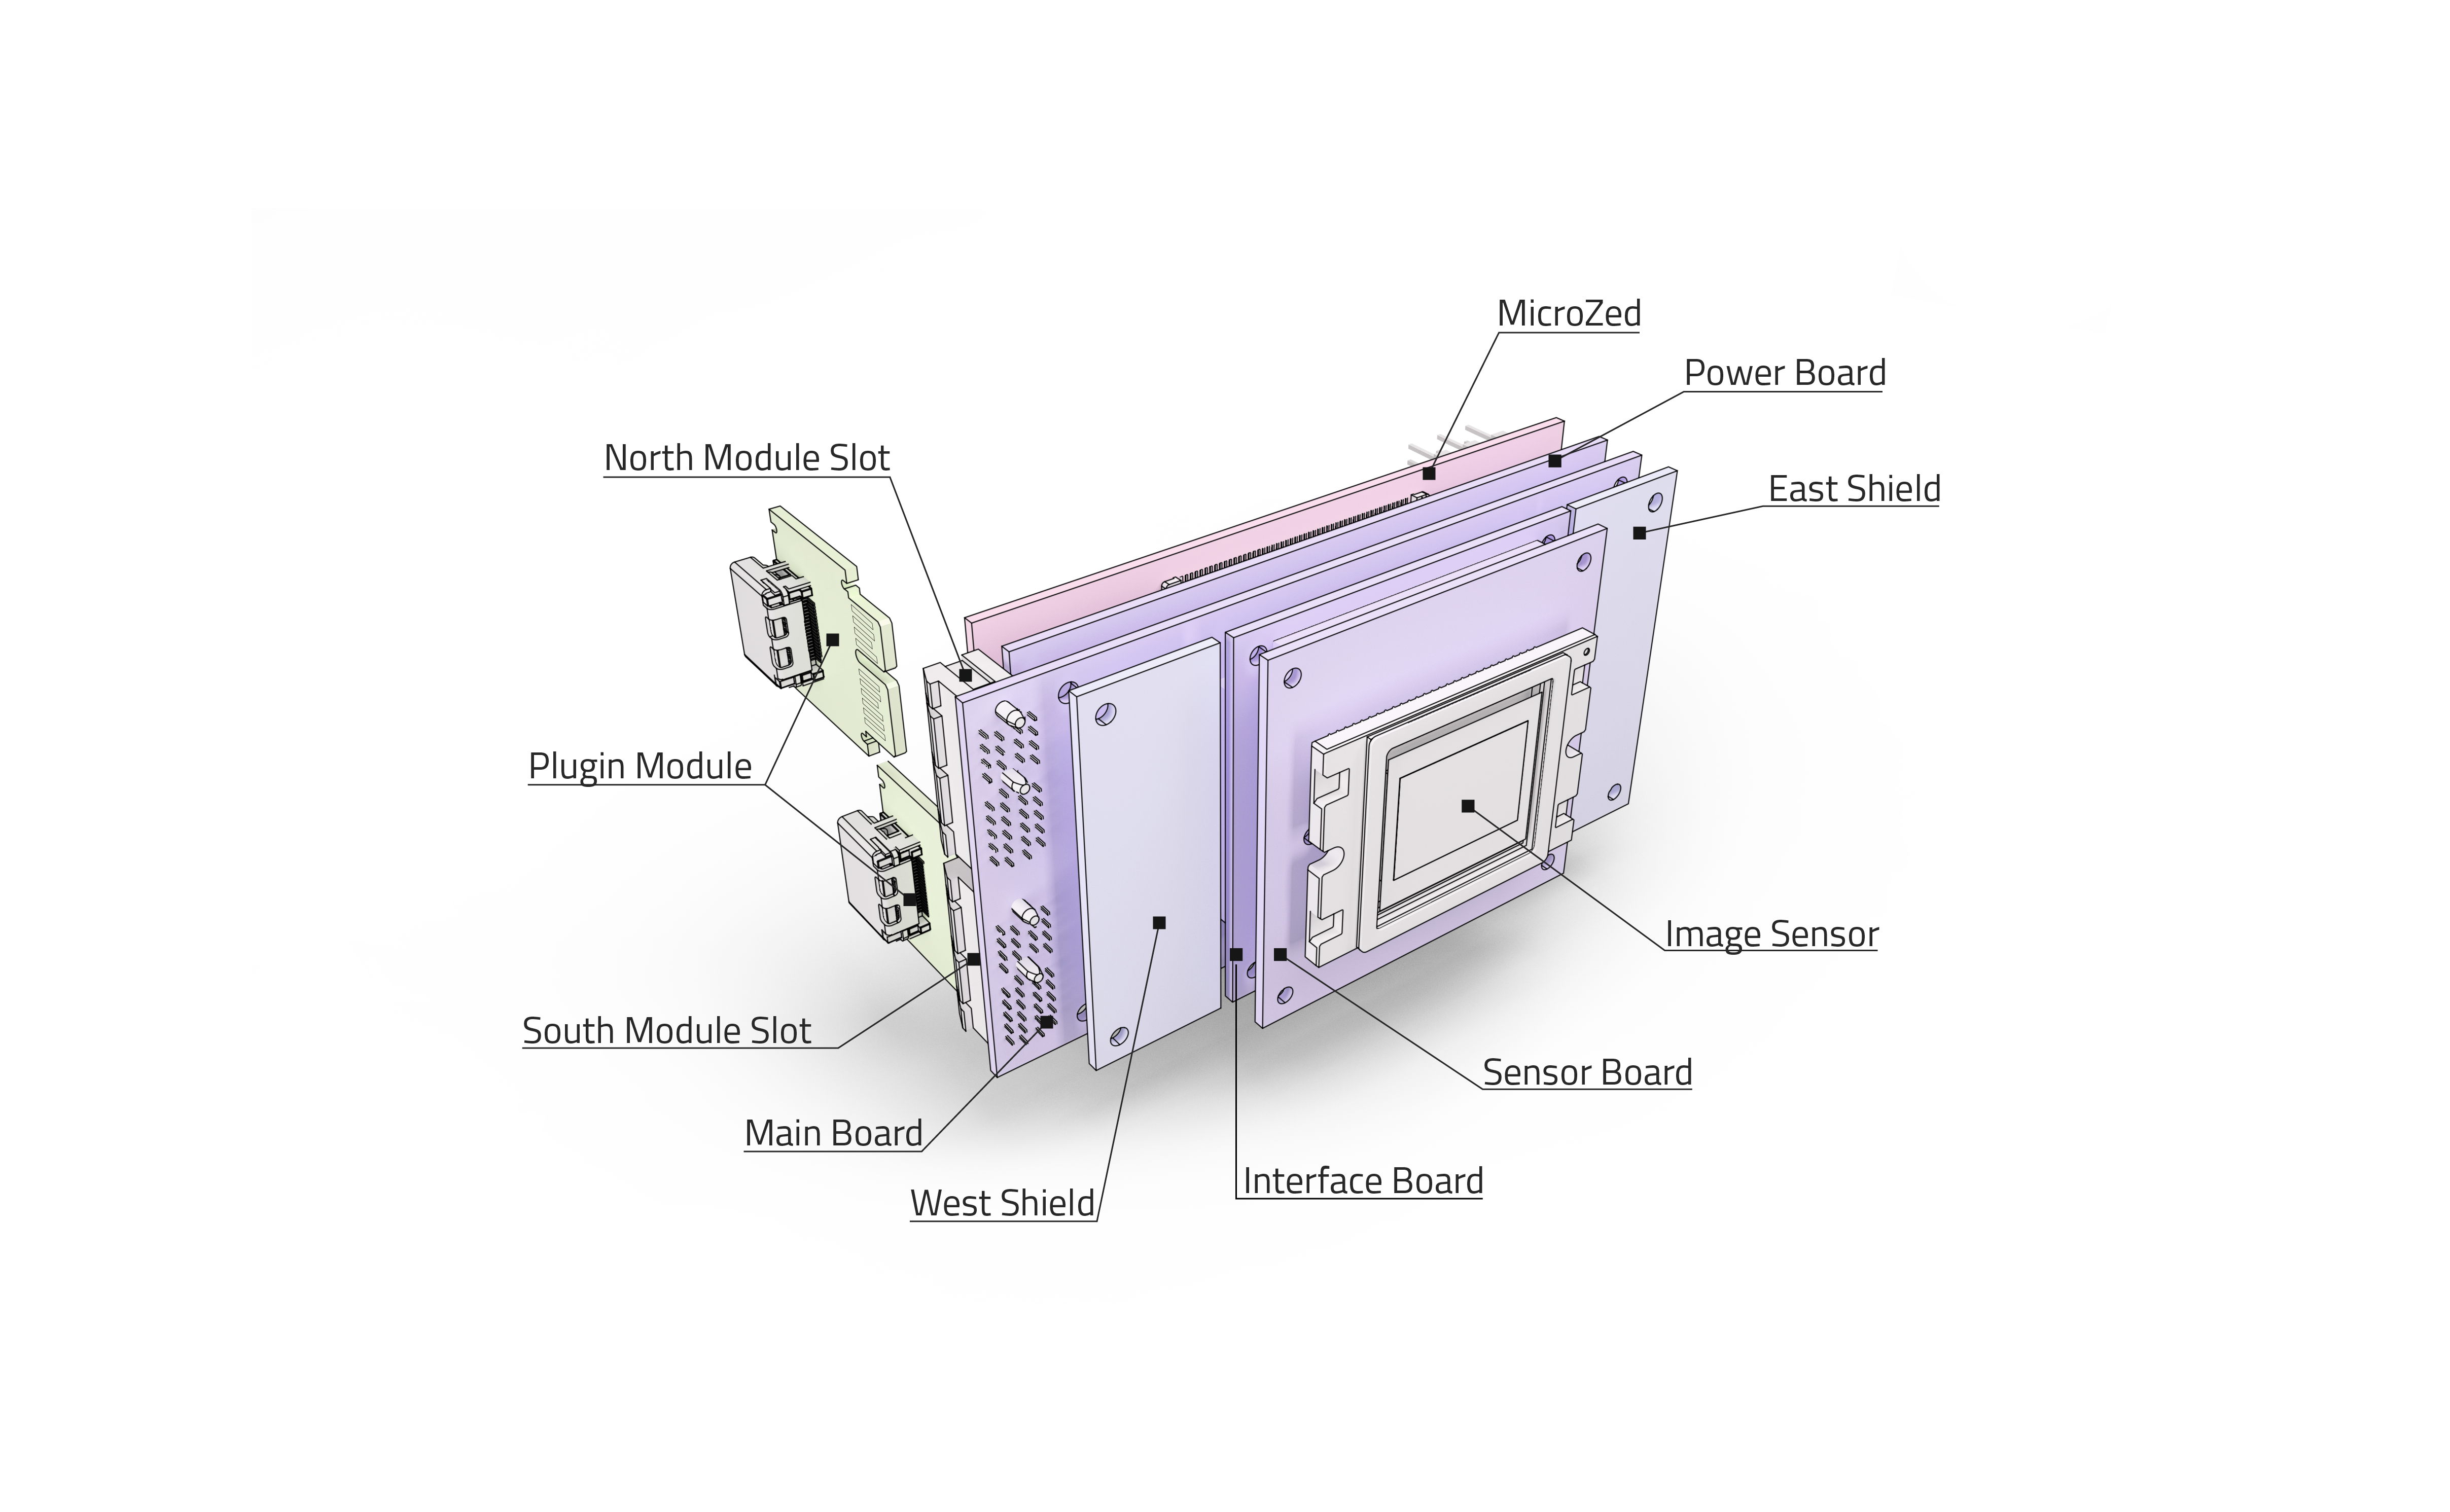
\includegraphics[height=10cm]{images/PCB_grey_new_pastel_labels-01}
\end{center}

Above: Version 5 of the camera's PCB stack layout.\\





\subsubsection{AXIOM Beta CMV12K THT Sensor Board}




For board revions see - \href{https://wiki.apertus.org/index.php/Beta_CMV12K_THT_Sensor_Board}{https://wiki.apertus.org/index.php/Beta\_CMV12K\_THT\_Sensor\_Board}





\subsubsection{AXIOM Beta Main Board}

The AXIOM Beta Mainboard deals with interfacing the plugin modules and shields and therefore acts as a kind of data crossroad.\\

The purpose of the two Lattice FPGAs (the so called routing fabrics) is to handle all the low speed GPIO stuff required for plugin modules, shields and CSO without sacrificing valuable Zynq GPIOs.\\

\begin{center}
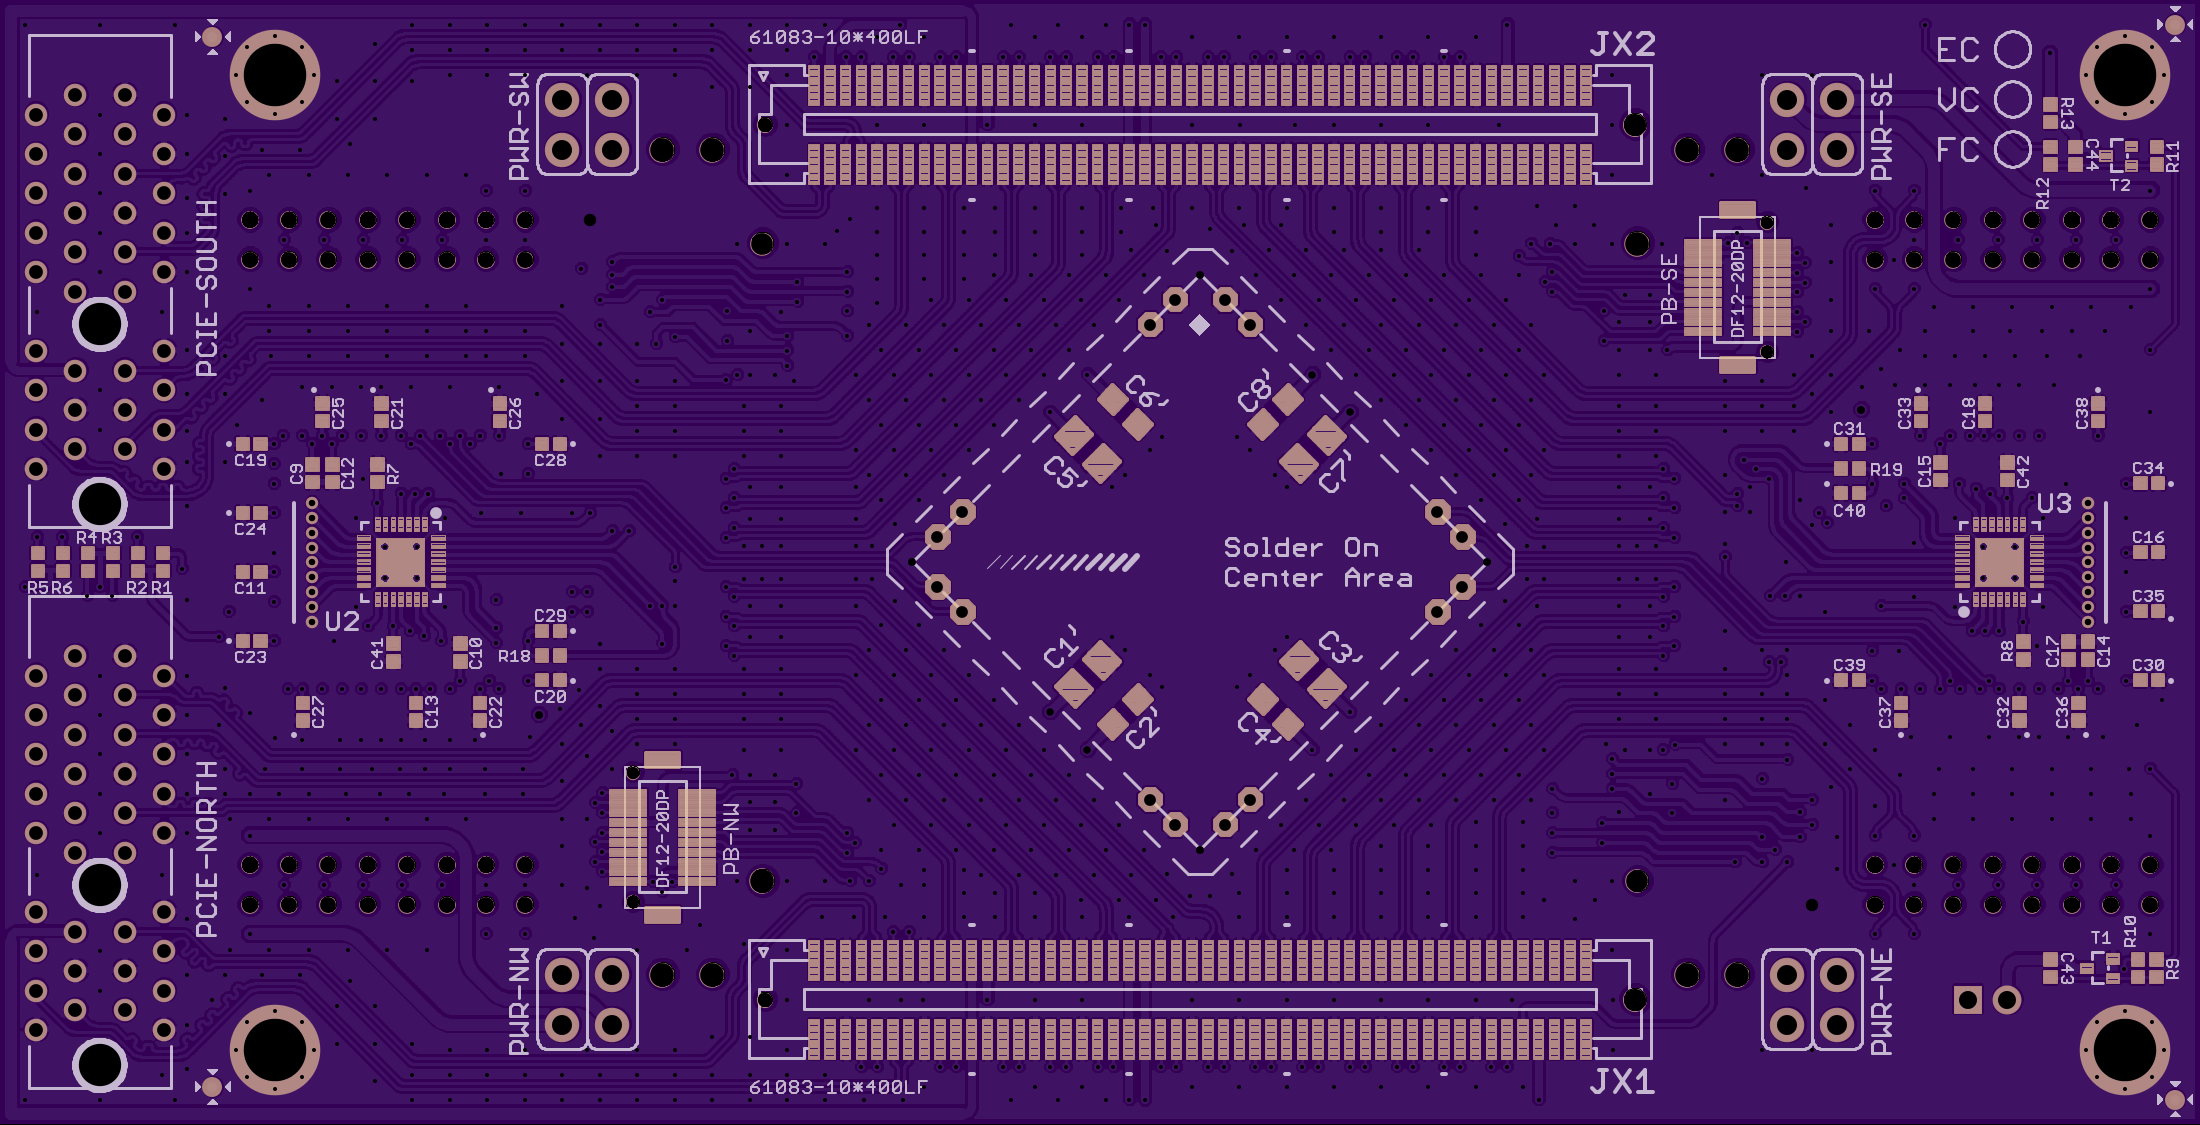
\includegraphics[height=6cm]{images/Beta_Main_Board_Top}
\end{center}

\begin{center}
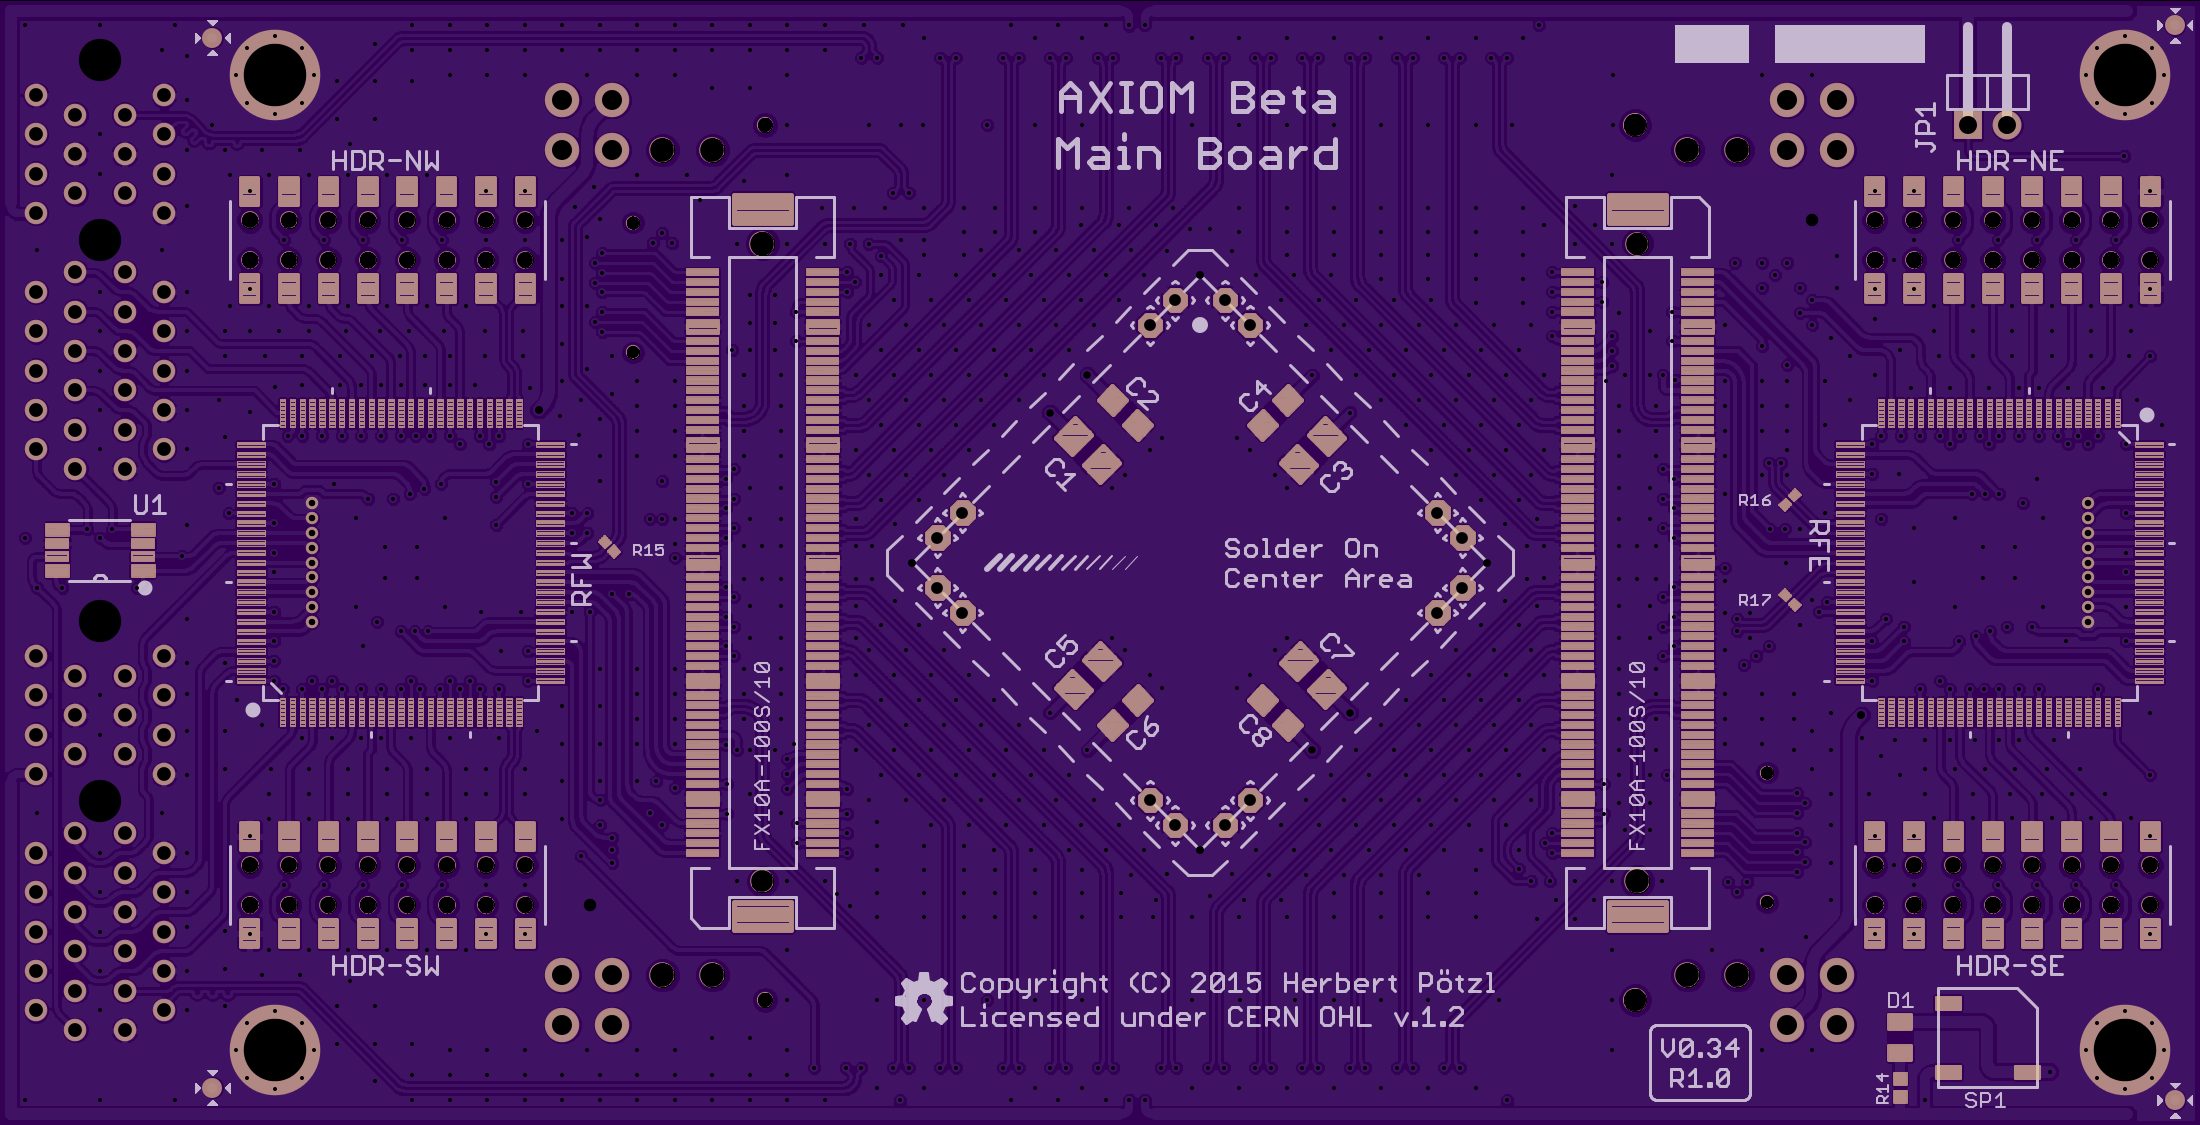
\includegraphics[height=9cm]{images/Beta_Main_Board_Bottom}
\end{center}

Beta Mainboard PCB populated with components:\\






\subsubsection{AXIOM Beta Power Board}

The AXIOM Beta Power Board PCB is the last board in the stack before the MicroZed™. It generates all the different supply voltages for the chips and logic on the other PCB’s inside the camera. It also monitors currents so that it can estimate remaining power based on the recorded consumption. In the current revision of the camera a predefined set of supply voltages matching the current application with the rest of the camera have been generated, in the future however, it will be possible for users to dynamically reconfigure voltages according to their needs through the camera’s software. 



Beta Power Board PCB populated with components:\\





For board revions see - \href{https://wiki.apertus.org/index.php/Beta_Power_Board}{https://wiki.apertus.org/index.php/Beta\_Power\_Board}.\\


\paragraph{Calibrating Voltages}\mbox{}\\

This describes the process required when factory assembling the power board hardware in the AXIOM Beta stack.\\

\consoleCommand{./power\_init.sh} 

\consoleCommand{./power\_on.sh} 

Wait a little...\\

\consoleCommand{./pac1720\_info.sh} 

This will output something like: 

\begin{lstlisting}[language=bash,morekeywords=$,keywordstyle=\bfseries,frame=none,xleftmargin=.25in,belowskip=2em, aboveskip=2em]
    ZED\_5V          4.8828 V [1f40]         +10.1562 mV [104]   +677.08 mA
    BETA\_5V         4.8828 V [1f40]          +1.2891 mV [021]    +85.94 mA
    HDN             3.2812 V [1500]          +0.0000 mV [000]     +0.00 mA
    PCIE\_N\_V        3.2422 V [14c0]          +0.0000 mV [000]     +0.00 mA
    HDS             3.2031 V [1480]          +0.0000 mV [000]     +0.00 mA
    PCIE\_S\_V        3.2422 V [14c0]          +0.0000 mV [000]     +0.00 mA
    RFW\_V           3.2422 V [14c0]          -0.0391 mV [fff]     -2.60 mA
    IOW\_V           3.2617 V [14e0]          +0.0000 mV [000]     +0.00 mA
    RFE\_V           3.2422 V [14c0]          +0.0000 mV [000]     +0.00 mA
    IOE\_V           3.2812 V [1500]          +0.0000 mV [000]     +0.00 mA
    VCCO\_35         2.4219 V [ f80]          -0.0391 mV [fff]     -2.60 mA
    VCCO\_13         2.4609 V [ fc0]          +0.0000 mV [000]     +0.00 mA
    PCIE\_IO         2.4609 V [ fc0]          -0.0781 mV [ffe]     -5.21 mA
    VCCO\_34         2.4609 V [ fc0]          +0.9766 mV [019]    +65.10 mA
    W\_VW            2.7734 V [11c0]          +0.0000 mV [000]     +0.00 mA
    N\_VW            2.8125 V [1200]          +0.0000 mV [000]     +0.00 mA
    N\_VN            2.7734 V [11c0]          -0.0391 mV [fff]     -2.60 mA
    N\_VE            2.8516 V [1240]          +0.0000 mV [000]     +0.00 mA
    E\_VE            2.6953 V [1140]          -0.0391 mV [fff]     -2.60 mA
    S\_VE            2.8516 V [1240]          +0.0000 mV [000]     +0.00 mA
    S\_VS            2.7344 V [1180]          -0.0391 mV [fff]     -2.60 mA
    S\_VW            2.8516 V [1240]          -0.0781 mV [ffe]     -5.21 mA
\end{lstlisting}

Now run: \\

\consoleCommand{watch -n 0.2 ./pac1720\_info.sh} 

... which will display the voltages in a clear screen and constantly update the values until you press CTRL+C.\\

The PCB labels and the labels in the CLI correspond like the following: 

\begin{lstlisting}[language=bash,morekeywords=$,keywordstyle=\bfseries,frame=none,xleftmargin=.25in,belowskip=2em, aboveskip=2em]
    WW = W\_VW
    NW = N\_VW
    NN = N\_VN
    NE = N\_VE
    SW = S\_VW
    SS = S\_VS
    SE = S\_VE
    EE = E\_VE
\end{lstlisting}

Use a tiny screwdriver and adjust the trimmers on the PCB until your values look like this:

\begin{lstlisting}[language=bash,morekeywords=$,keywordstyle=\bfseries,frame=none,xleftmargin=.25in,belowskip=2em, aboveskip=2em]
    W\_VW          	2.4609 V [ fc0] 	 -0.0391 mV [fff]     -2.60 mA
    N\_VW          	3.2422 V [14c0] 	 +0.0000 mV [000]     +0.00 mA
    N\_VN          	1.8750 V [ c00] 	 -0.0391 mV [fff]     -2.60 mA
    N\_VE          	3.2617 V [14e0] 	 +0.0000 mV [000]     +0.00 mA
    E\_VE          	3.2812 V [1500] 	 +0.0391 mV [001]     +2.60 mA
    S\_VE          	1.9922 V [ cc0] 	 +0.0000 mV [000]     +0.00 mA
    S\_VS          	2.9883 V [1320] 	 -0.0391 mV [fff]     -2.60 mA
    S\_VW          	1.9531 V [ c80] 	 -0.1172 mV [ffd]     -7.81 mA
\end{lstlisting}





\subsubsection{Beta Power Adapter Board}

Overview text required.

\begin{center}
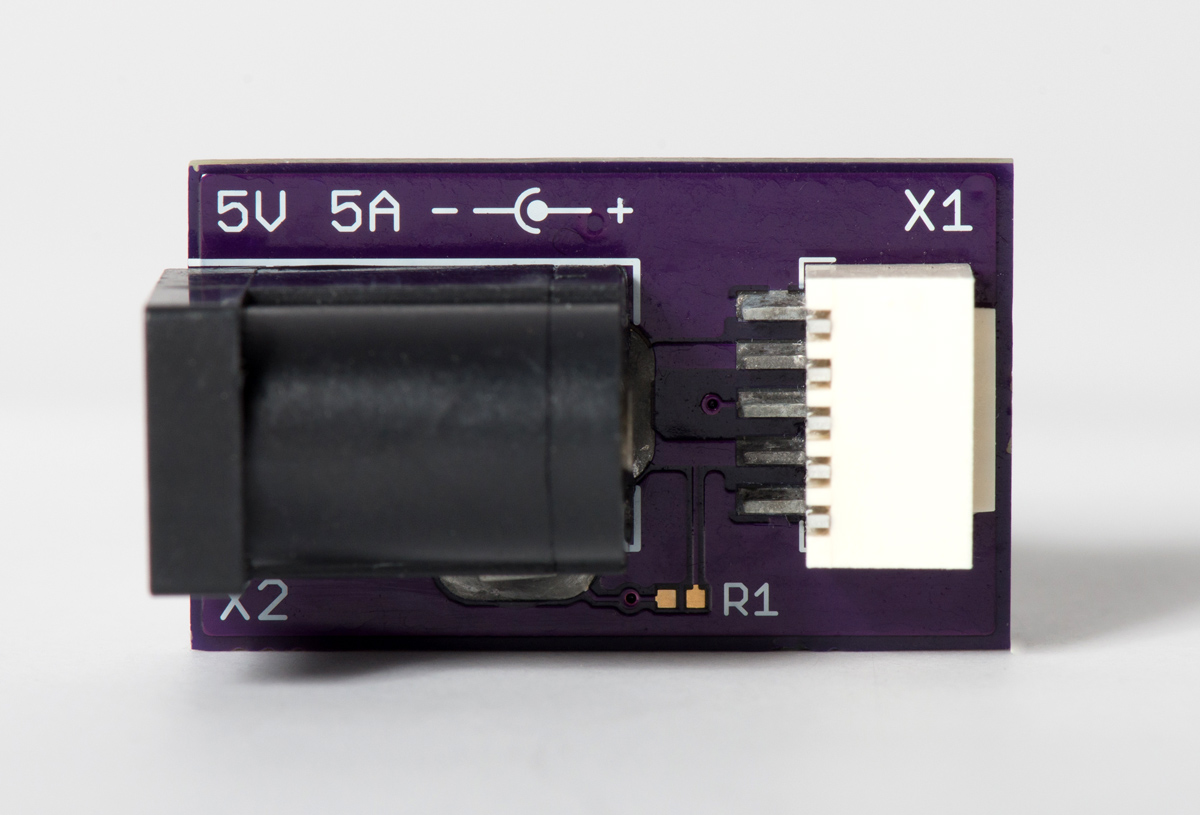
\includegraphics[height=6cm]{images/Power-adapter-02}
\end{center}

\begin{center}
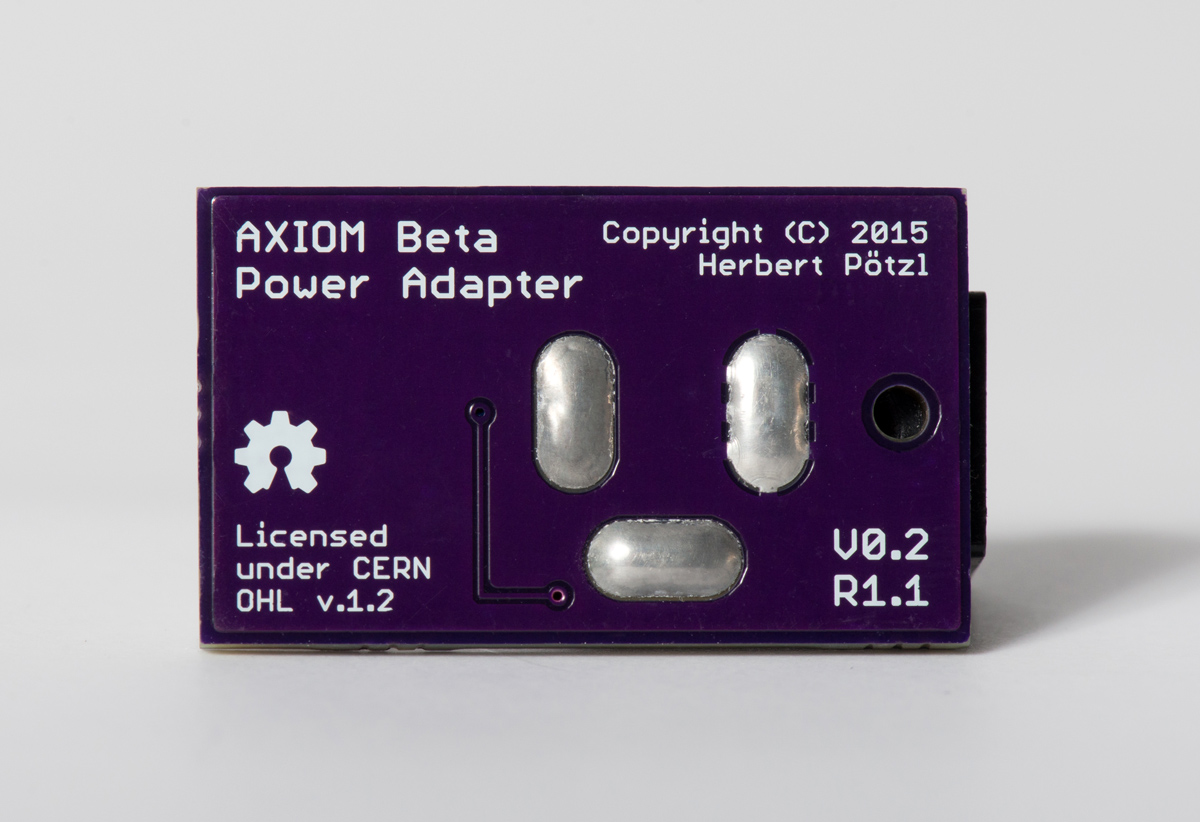
\includegraphics[height=6cm]{images/Power-adapter-01}
\end{center}

For board revions and concepts see - \href{https://wiki.apertus.org/index.php/Beta_Power_Adapter_Board}{https://wiki.apertus.org/index.php/Beta\_Power\_Adapter\_Board}.\\







\subsubsection{AES-Z7MB-7Z020-SOM-G MicroZed}

MicroZed is a low-cost development board based on the Xilinx Zynq®-7000 All Programmable SoC. Its unique design allows it to be used as both a stand-alone evaluation board for basic SoC experimentation, or combined with a carrier card as an embeddable system-on-module (SOM). MicroZed contains two I/O headers that provide connection to two I/O banks on the programmable logic (PL) side of the Zynq-7000 All Programmable SoC device. In stand-alone mode, these 100 PL I/O are inactive. When plugged into a carrier card, the I/O are accessible in a manner defined by the carrier card design.\\

\href{https://wiki.apertus.org/index.php/File:AES-Z7MB-7Z020-SOM-G_MicroZed_Datasheet.pdf}{Datashet}.\\


\begin{center}
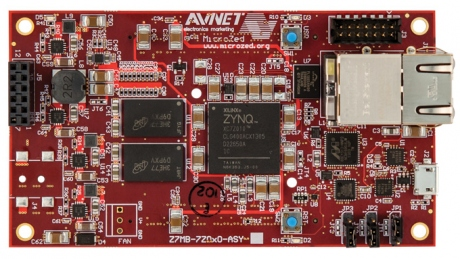
\includegraphics[height=8cm]{images/MicroZed}
\end{center}


Features:\\


- SoC XC7Z010-1CLG400C\\
    
    
Memory:\\

- 1 GB of DDR3 SDRAM\\
- 128 Mb of QSPI Flash\\
- Micro SD card interface\\


Communications:\\

- 10/100/1000 Ethernet\\
- USB 2.0\\
- USB-UART\\

User I/O (via dual board-to-board connectors):\\

- 7Z010 Version\\
- 100 User I/O (50 per connector)\\
- Configurable as up to 48 LVDS pairs or 100 single-ended I/O\\

Other:\\

- 2x6 Digilent Pmod® compatible interface providing 8 PS MIO connections for user I/O\\
- Xilinx PC4 JTAG configuration port\\
- PS JTAG pins accessible via Pmod\\
- 33.33 MHz oscillator\\
- User LED and push switch\\


Wiki - \href{https://wiki.apertus.org/index.php/AES-Z7MB-7Z020-SOM-G}{https://wiki.apertus.org/index.php/AES-Z7MB-7Z020-SOM-G}.\\







\subsubsection{Shields}

Overview text required.\\

\paragraph{Beta Debug Shield}\mbox{}\\

2x10 GPIO banks as LED indicators plus two power LEDs. 4 LVDS pairs routed to external connectors JP1/JP2 (2 LVDS plus one GND each). 

\begin{center}
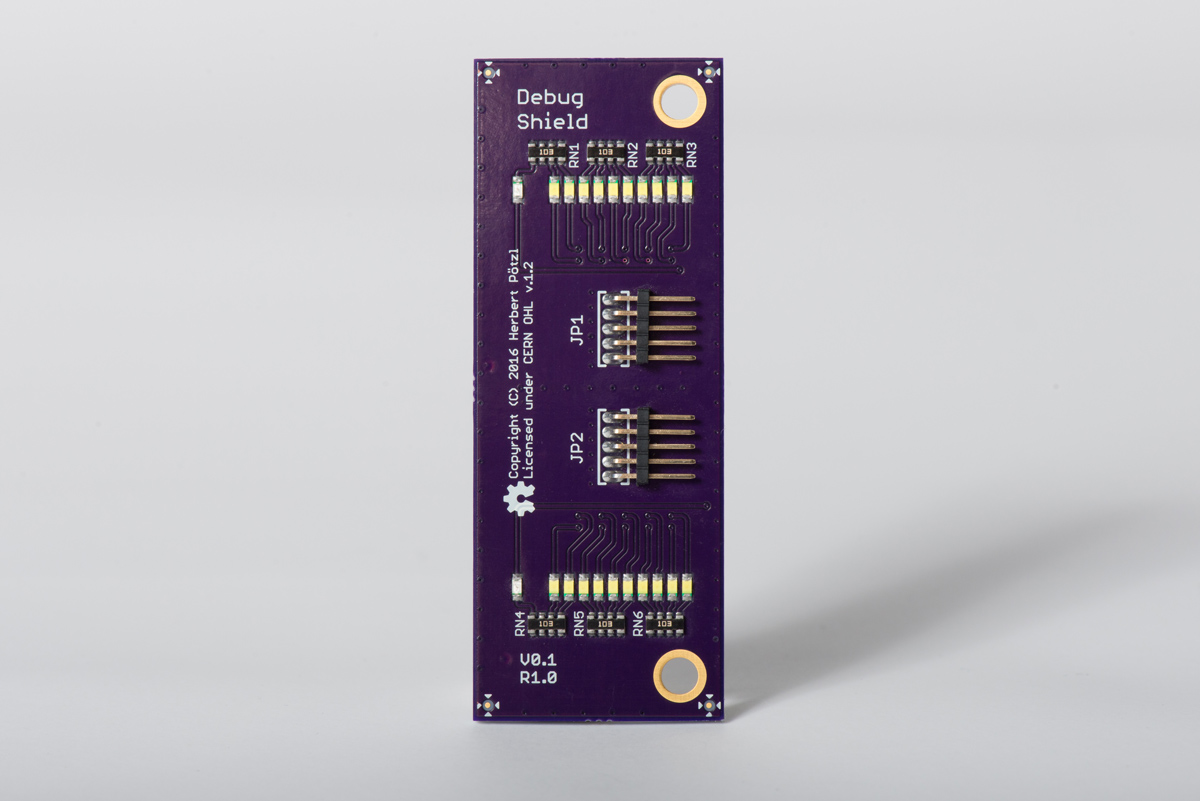
\includegraphics[height=6cm]{images/Debug-shield-bot01}
\end{center}

\begin{center}
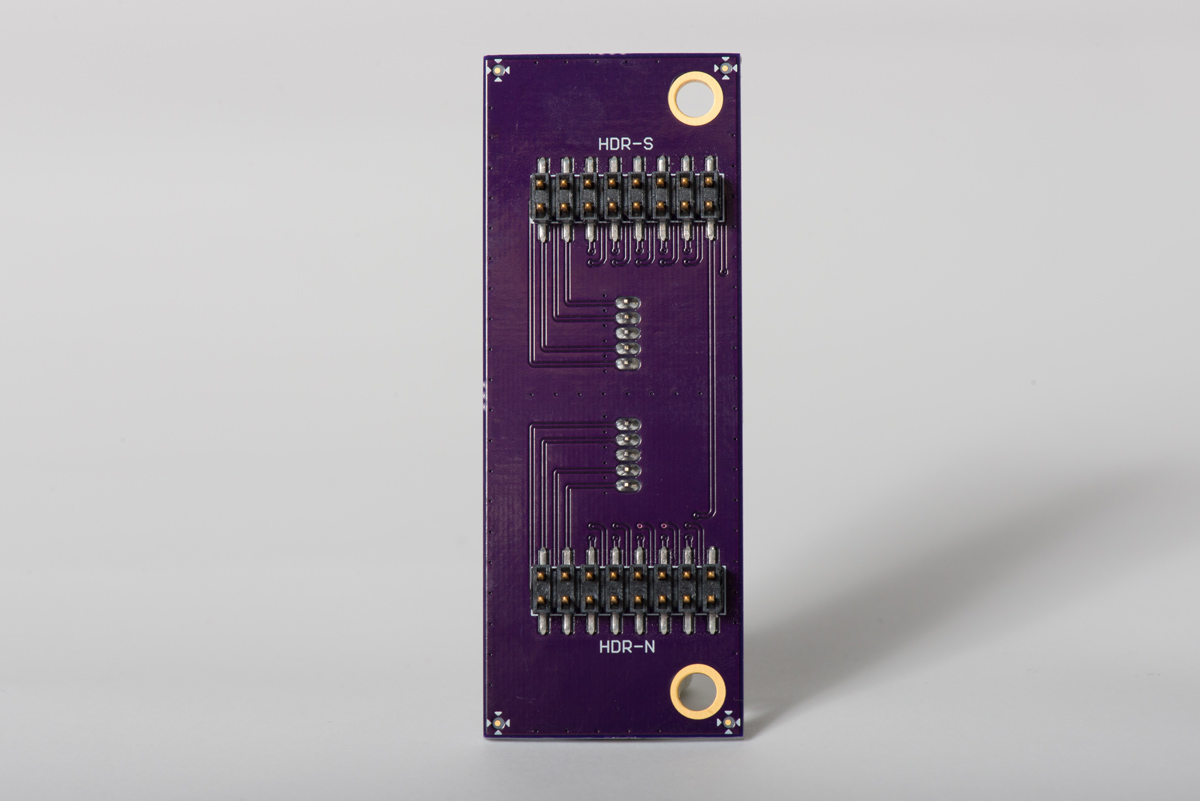
\includegraphics[height=6cm]{images/Debug-shield-top01}
\end{center}

For board revions see - \href{https://wiki.apertus.org/index.php/Beta_Debug_Shield}{https://wiki.apertus.org/index.php/Beta\_Debug\_Shield}.\\







\subsubsection{Plugin Modules}

Overview text required.

\paragraph{Beta HDMI Plugin Module}\mbox{}\\

This module provides one 1080p60 HDMI output stream via 4 LVDS channels directly from the Zynq on the Microzed 




For board revions, dimensions and other files see - \href{https://wiki.apertus.org/index.php/Beta_HDMI_Plugin_Module}{https://wiki.apertus.org/index.php/Beta\_HDMI\_Plugin\_Module}.\\


\paragraph{Beta 1x PMOD Plugin Module }\mbox{}\\

Overview text required.\\

\begin{center}
\includegraphics[height=6cm]{images/1xpmodbot}
\end{center}

\begin{center}
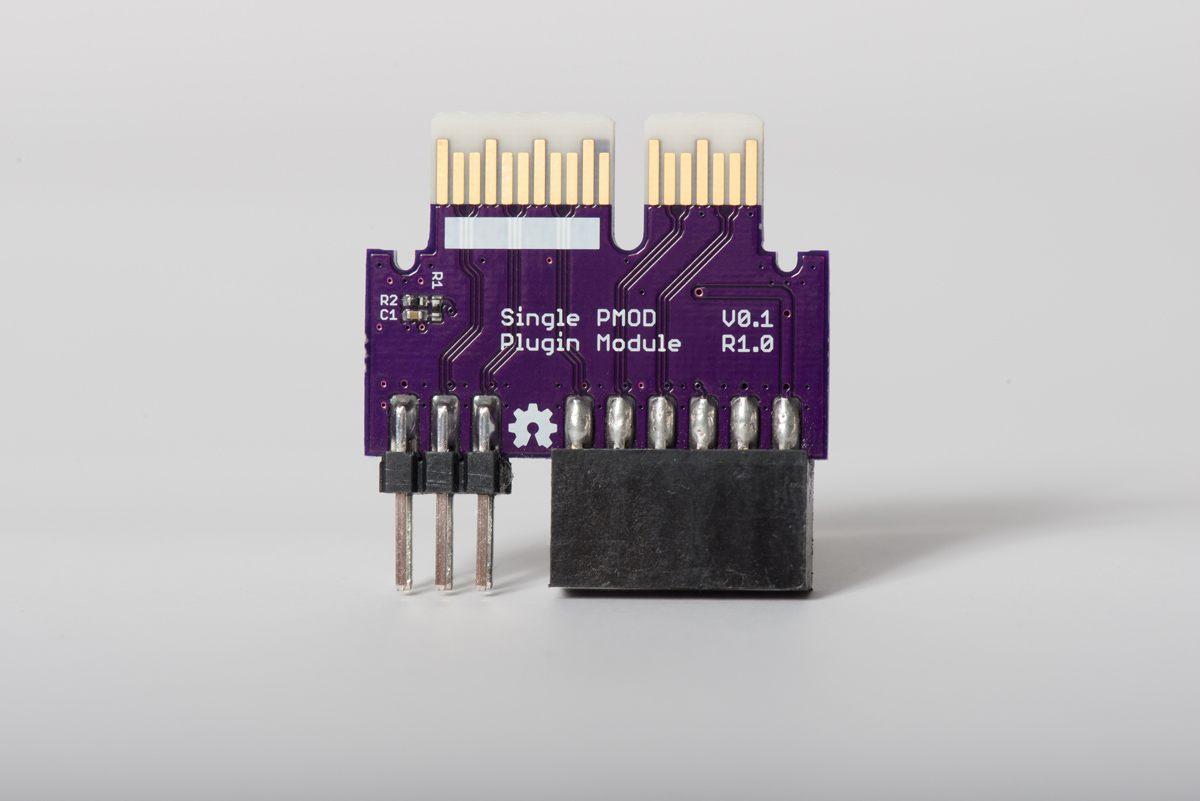
\includegraphics[height=6cm]{images/1xpmodtop}
\end{center}


For board revions see - \href{https://wiki.apertus.org/index.php/Beta_1x_PMOD_Plugin_Module}{https://wiki.apertus.org/index.php/Beta\_1x\_PMOD\_Plugin\_Module}.\\



\paragraph{4K HDMI Plugin Module}\mbox{}\\

Work in progress.

\subsubsection{EEPROM}

All PCBS we created for the AXIOM Beta (beside the AXIOM Beta Mainboard) have an onboard \href{https://en.wikipedia.org/wiki/EEPROM}{EEPROM}. These chips provide between 4KB and 16KB of non-volatile memory.\\

Our primary use for these EEPROMs is to store unique identifiers for each board/type. In a modular stack of PCBs the camera firmware can read the EEPROMs of each PCB and identify which boards, versions and revisions are attached (as different board versions might need different drivers/firmware elements).\\

\paragraph{Proposed Unique ID Structure}\mbox{}\\

2 byte board type identifier (65.536 possible values): 

\consoleCommand{00 - AXIOM Beta Powerboard
01 - AXIOM Beta Interface Board
02 - AXIOM Beta Sensor Frontend
03 - AXIOM Beta Single Slot Plugin Module
04 - AXIOM Beta Dual Slot Plugin Module
05 - AXIOM Beta Low Speed Shield
06 - AXIOM Beta Medium Speed Shield} 

1 byte board output identifier: 

\consoleCommand{number of output interfaces} 

1 byte board active/passive identifier.\\

4 byte board current draw range identifier\\

\consoleCommand{    2 bytes typical low end range in mA
    2 bytes typical high end range in mA}
    
2 byte board length in mm.\\
1 byte number of used LVDS lanes.\\
1 byte number of used GPIO channels.\\
2 byte board identifier:

\consoleCommand{00 - AXIOM Beta Powerboard
01 - AXIOM Beta Interface Dummy
02 - AXIOM Beta Interface Board
03 - AXIOM Beta CMV12000 ZIF Sensor Frontend
04 - AXIOM Beta CMV12000 Socket Sensor Frontend
05 - AXIOM Beta 1x HDMI Plugin Module
06 - AXIOM Beta 3x Displayport Plugin Module
07 - AXIOM Beta 1x PMOD Plugin Module
08 - AXIOM Beta 3x PMOD Plugin Module
09 - AXIOM Beta 1x HDMI IN Plugin Module
0A - AXIOM Beta Dual Riser Plugin Module
0B - AXIOM Beta Debug Shield}

2 byte board version identifier - (ASCII A.BC corresponding to label printed on PCB)\\

2 byte board revision identifier - (ASCII A.BC corresponding to label printed on PCB)\\


128 byte UUID 




\subsection{Power Supply}
\subsubsection{AC Power Supply}
\subsubsection{DC Power Supply}
\subsubsection{Active Battery Mount}
\subsection{Enclosure}
\subsubsection{Skeleton}
\subsubsection{Simple Enclosure}
\subsubsection{Transparent Acrylic Enclosure}
\subsection{Optical Information}
\subsubsection{Lens Mount}
\subsubsection{Lens Mount Overviews}
\subsubsection{Infra Red / Ultra Violet Cut-off Filter}
\subsubsection{Optical Low-pass Filter (OLPF)}
